\chapter{Wprowadzenie teoretyczne}
\label{cha:wprowadzenieTeoretyczne}

%---------------------------------------------------------------------------

\section{Przetwarzanie języka naturalnego}
\label{sec:przetwarzanieJezykaNaturalnego}


Zgodnie z definicją, przetwarzanie języka naturalnego (zwanego dalej jako NLP - ang. Natural Language Processing) opiera się na rozpoznawaniu, rozumieniu i produkowaniu języka naturalnego. Za początki NLP uznaje się już lata pięćdziesiąte ubiegłego wieku - wtedy nastąpiła publikacją słynnego Testu Turinga. Przedstawia on sytuację w której maszyna oraz człowiek komunikują się tylko za pomocą tekstu pisanego. Turing twierdzi, że jeśli zewnętrzny obserwator po konwersacji z każdym z podmiotów nie będzie w stanie stwierdzić, który z nich jest człowiekiem - wtedy maszyna zalicza test i wykazuje zachowanie inteligentne. Pomimo wielu prób, nadal nie można jednoznacznie stwierdzić, czy jakakolwiek maszyna zaliczyła test Turinga. Podchodząc do rozwiązania wspomnianego testu, nietrudno wywnioskować jest, że kluczem do jego rozwiązania będzie rozumienie języka naturalnego (ludzkiego) przez maszynę. 

Przez ponad 30 lat od definicji Testu Turinga rozwiązywanie problemów NLP bazowane było na złożonych zasadach definiowanych ręcznie w algorytmach. Dopiero lata 80’ przyniosły znaczny postęp w tej dziedzinie. W związku z wzrostem mocy obliczeniowej komputerów zaczęto używać metod uczenia maszynowego, które pozwalały na uzyskanie dużo lepszych wyników w rozwiązywaniu tych problemów. Jednym z modeli wykorzystywanych na początku było drzewo decyzyjne, które skutkowało w produkcji modelu złożonego z wielu instrukcji warunkowych, co miało wiele podobieństw z modelami bazującymi na definiowaniu zasad używanymi przed erą uczenia maszynowego w problemach NLP. Jednakże użycie tych metod pozwalało na automatyzację procesu tworzenia modelu, co znacznie ułatwiło dalszy rozwój. Od tego momentu duża część aplikacji i rozwiązań zbudowanych wokół problemu NLP opiera się na podejściu data-driven.

Problem NLP stał się również bardzo znaczący w kontekście powstania i rozwoju Internetu. W Internecie z upływem czasu znajduje się coraz więcej danych, z których ogromną ilość stanowią dane w formie tekstu. Rozwój metod NLP pozwala nam na efektywne przeszukiwanie zasobów w sieci. Działa to również w drugą stronę: dane pochodzące z Internetu są wykorzystywane do uczenia algorytmów NLP, co sprawia, że zasoby w sieci są coraz szybciej dostępne i lepiej uporządkowane.

W kolejnych podrozdziałach skupię się na opisach oraz analizie metod NLP w kontekście dużych zbiorów danych oraz podejściu data-driven.

\subsection{Zbieranie danych}

Pierwszą i niezbędną częścią tworzenia systemu rozwiązującego problem przetwarzania języka naturalnego podejściem data-driven jest zbieranie danych tekstowych. Ważnym aspektem tutaj jest jakość oraz ilość zebranych danych - będą one znacząco wpływać na skuteczność rozwiązania problemu. Idealny zbiór danych powinien zawierać reprezentatywne dane, jasno podzielone na kategorie/gatunki i w podobnej ilości dla każdej kategorii. Ta ostatnia cecha może stanowić spory problem przy budowaniu zbioru danych. Przykładowo budując system przypisujący dziedzinę nauki do wprowadzonego artykułu naukowego musimy zebrać dostateczną ilość reprezentatywnych artykułów oznaczonych konkretną dziedziną jakiej dotyczą. Musimy się liczyć z różną dostępnością artykułów z poszczególnych dziedzin. Rozwiązaniem jest odrzucenie części artykułów i zebranie dla każdej dziedziny tylko tylu, ile możemy znaleźć dla dziedziny z najmniejszą ilością artykułów, przy czym musimy pamiętać, że wielkość zestawu ma duży wpływ na skuteczność systemu.

Dane mogą być zbierane zarówno drogą manualną, jak i automatyczną. W celu pozyskania zbioru o wysokiej jakości często niezbędne jest zatrudnianie ekspertów z dziedziny lingwistyki, którzy własnoręcznie gromadzą i opisują dane. Obecnie raczej dużo częściej wykorzystywane są metody automatyczne, głównie ze względu na ilość danych jakie potrafią zgromadzić. Projekty osobistych asystentów (Apple Siri, Google Assistant itp.) i ich sukces dowodzą, że dane zebrane metodami automatycznymi znakomicie sprawdzają się przy uczeniu maszynowym i poleganie jedynie na metodach manualnych nie jest konieczne.

Unikniemy wielu problemów związanych z zbieraniem danych, jeśli wykorzystamy gotowe zestawy dostępne w sieci. Przykładem jest British National Corpus - posiada on wiele przykładów tekstu z gazet, magazynów, tekstów akademickich i innych rzetelnych źródeł. Każdy tekst podzielony jest na słowa z których każde jest oznaczone właściwą częścią mowy, formą i innymi parametrami zgodnymi ze standardem TEI \footnote{http://www.tei-c.org/}.


\subsection{Analiza i przetwarzanie danych}

Po etapie pozyskania danych bardzo ważnym procesem jest ich przetworzenie i właściwe oznaczenie. W obecnych czasach wykorzystuje się do tego raczej automatyczne narzędzia, które znacznie ograniczają czas i wysiłek włożony w cały proces przetwarzania języka naturalnego.

Przykładowe procesy stosowane przy przetwarzaniu tekstu:
\begin{enumerate}
    \item Lematyzacja lub stemming - ich celem jest mapowanie słowa z tekstu na ich formę kanoniczną. Jako rezultat słowa o takim samym znaczeniu, ale innej formie traktowane są jako jedno i to samo. Proces ten często prowadzi do utraty części informacji zawartych w tekście, lecz pozwala na prostsze przetwarzanie danych w dalszych etapach.

    \newpage
    \begin{lstlisting}[caption={Przykład lematyzacji},captionpos=b]
        are, be, am, is => be
        analyse, analysis, analyses => analyse
    \end{lstlisting}
    
    \item Tagowanie części mowy (ang. Part-of-speech tagging) - oznaczanie każdego wyrazu z jego częścią mowy.

    \begin{lstlisting}[caption={Przykład tagowania części mowy}]
        James => noun
        made => verb
    \end{lstlisting}
    
    \item Parsowanie - podobnie do parsowania języka programowania - tutaj także budujemy drzewo syntaktyczne ze zdania w języku naturalnym. Jest ono trudniejszym procesem od dwóch poprzednich, ponieważ wymaga bardziej zaawansowanej wiedzy z dziedziny lingwistyki.

    \begin{figure}[H]
    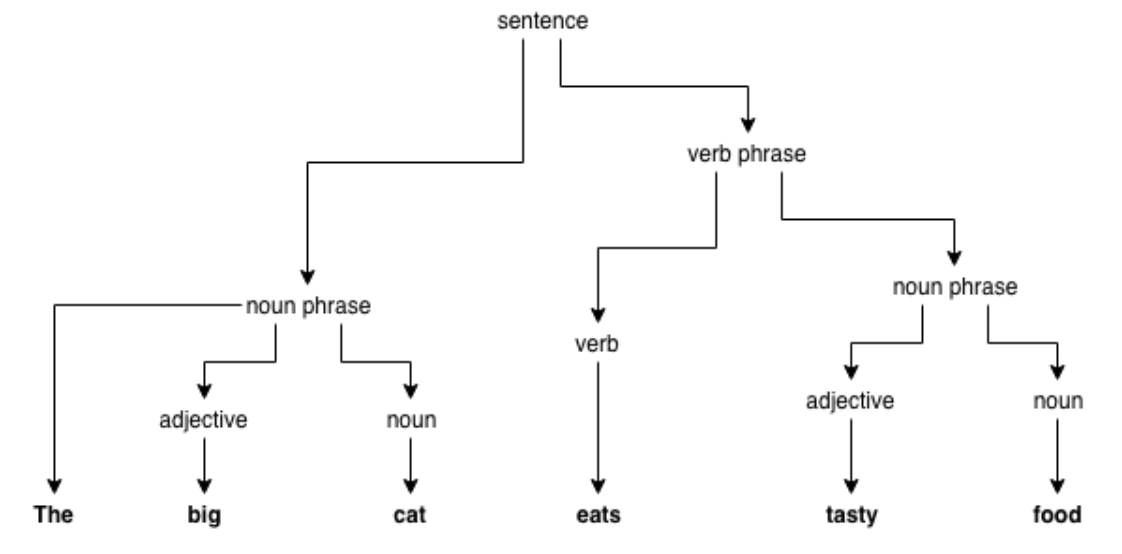
\includegraphics[width=10cm]{parsing_example.png}
    \centering
    \caption{Przykład parsowania zdania}
    \end{figure} 
    
\end{enumerate}

Wstępnie przetworzony tekst jest łatwiejszy do analizy - niektóre z popularnych metod analizy tekstu to:

\begin{enumerate}
    \item Zgodność (ang. concordance) - badanie kontekstu danego słowa. Jako rezultat dostajemy różne otoczenia w jakich słowo występuje w zbiorze danych.
    
    \item Częstość występowania słowa - uzyskanie listy najczęściej występujących słów w naszym zbiorze.

    \item Szukanie sekwencji słów które często występują obok siebie (ang. collocation extraction).

\end{enumerate}

\subsubsection{N-gram}

N-gramem jest nazywana sekwencja kolejnych n elementów występujących po sobie w przetwarzanej próbce. W przypadku przetwarzania języka naturalnego najczęściej bierze się pod uwagę kolejne słowa. Dzięki analizie n-gramów znamy kontekst występowania danego słowa, lub jesteśmy w stanie przewidzieć jakie słowo może pojawić się dalej. Weźmy pod uwagę przykładowe zdanie: “to be or not to be”. Rozkład na modele n-gram może wyglądać następująco:

\begin{enumerate}
    \item unigramy: [ ‘to’, ‘be’, ‘or’, ‘not’, ‘to’, ‘be’ ] 
    \item bigramy: [ ‘to be’, ‘be or’, ‘or not’, ‘not to’, ‘to be’ ]
    \item trigramy: [‘to be or’, ‘be or not’, ‘or not to’, ‘not to be’ ]
\end{enumerate}

Przy przetwarzaniu tekstu n-gramy wydają się bardzo przydatnym modelem pod kątem analizy kontekstu. Polegając jedynie na unigramach nie będziemy w stanie wyciągnąć wielu znaczących informacji z tekstu takich jak negacje  (‘good’ vs ‘not good’) lub zaprzeczenia (‘do’ vs ‘do not’).

\subsubsection{Bag of words}

Aby umożliwić przetwarzanie tekstu przez algorytmy uczenia maszynowego trzeba sprowadzić go do reprezentacji macierzowej. Bag of words jest jednym z najprostszych modeli pozwalających wykonać to zadanie. Każdy element macierzy wyprodukowanej przez ten model odpowiada liczbie wystąpień jednego słowa z tekstu.

\begin{verbatim}
    Dane wejściowe: “Machine learning gains more and more popularity.”
    Bag of words: { 
        “machine”: 1, 
        “learning”: 1, 
        “gains”: 1, 
        “more”: 2, 
        “and”: 1, 
        “popularity”: 1 
    }
\end{verbatim}

\subsubsection{TF-IDF}

Rozszerzeniem modelu Bag of words jest Term Frequency - Inverse Document Frequency \footnote{https://pl.wikipedia.org/wiki/TFIDF}. Do klasycznego Bag of words dodaje on wagę do każdego ze słów. Słowo często występujące w jednym dokumencie, a rzadko w innych będzie miało wyższą wagę, natomiast słowo występujące równie często w analizowanym dokumencie, w reszcie zostanie oznaczone niższą wagą.

%---------------------------------------------------------------------------

\section{Uczenie maszynowe}
\label{sec:uczenieMaszynowe}

Algorytmy uczenia maszynowego pozwalają nam na tworzenie rozwiązań bazujących na doświadczeniach i przykładach, zamiast na jawnie zaprogramowanych zasadach. Algorytmy uczenia maszynowego wymagają często większej mocy obliczeniowej niż standardowe rozwiązania, ponieważ bazują na dużych zestawach danych wejściowych. 

Rodzaje algorytmów uczenia maszynowego:

\begin{enumerate}
    \item Uczenie nadzorowane - zasilane przez opisane dane na podstawie których algorytm jest uczony i dopiero po wykonaniu tego procesu jest on gotowy do użycia.

    \item Uczenie nienadzorowane - algorytmy zasilane są nieopisanymi danymi, które mają uporządkować poprzez znalezienie podobnych cech pośród danych wejściowych.
\end{enumerate}

Przykład: Na podstawie rozmiaru buta i wzrostu mamy zadanie określić płeć człowieka.
W uczeniu nadzorowanym wizualizacja zestawu danych może wyglądać następująco:

    \begin{figure}[H]
    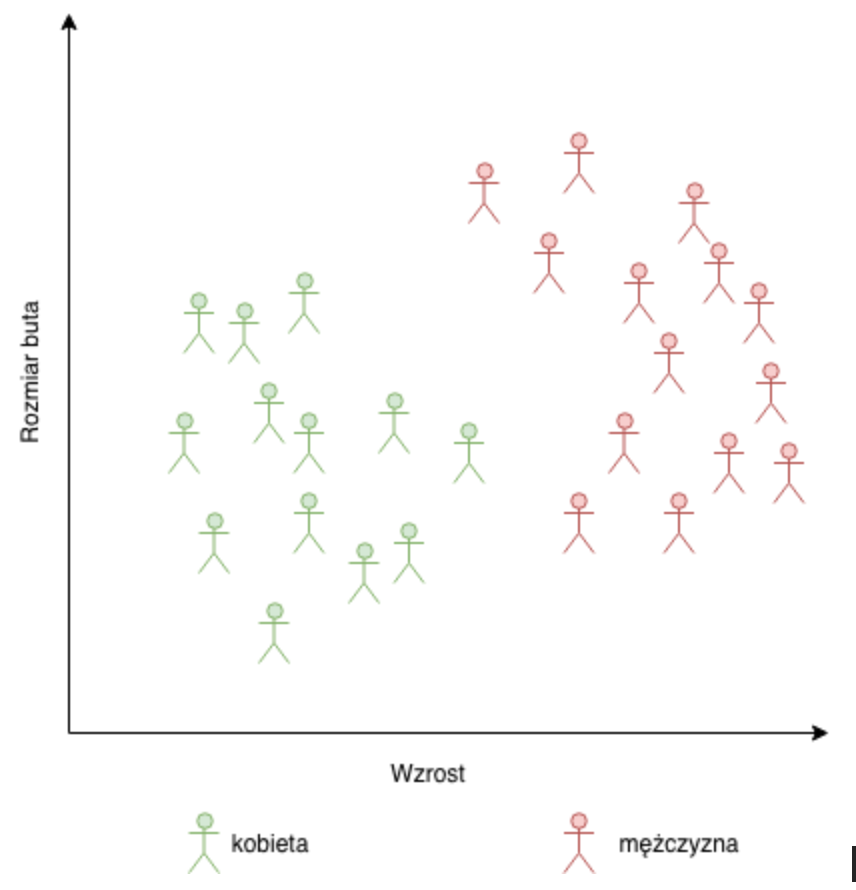
\includegraphics[width=8cm]{supervised_dataset_example.png}
    \centering
    \caption{Wizualizacja przykładowego zbioru uczącego w uczeniu nadzorowanym}
    \end{figure}
    
Wykorzystując algorytm uczenia nienadzorowanego, nasze dane nie są opisane. W podanym przykładzie możemy wykorzystać automatyczną klasteryzację.

    \begin{figure}[H]
    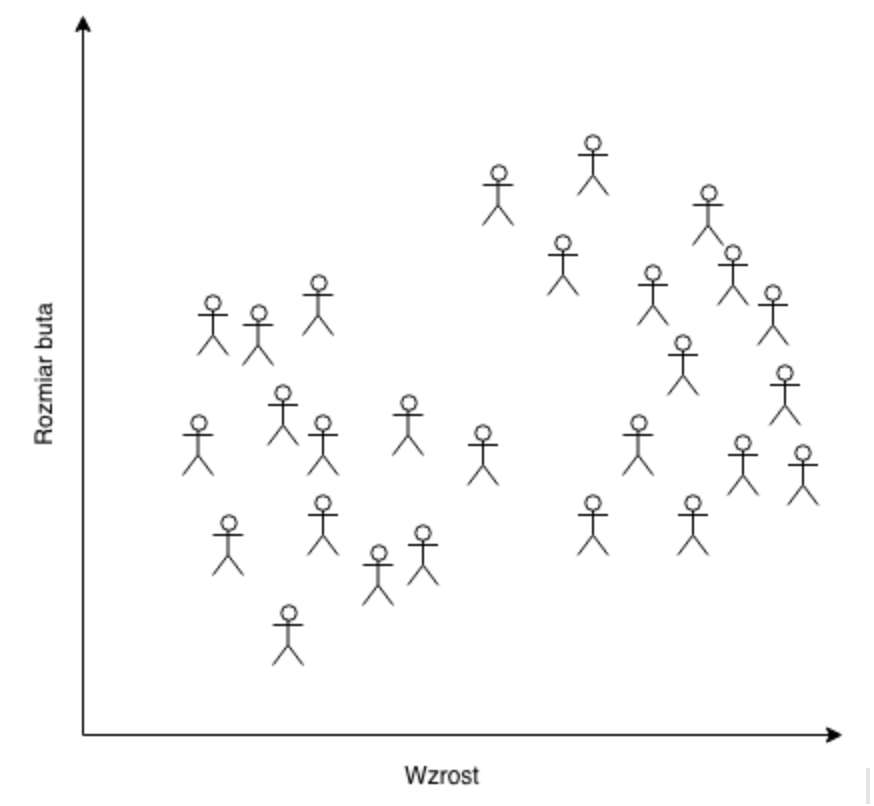
\includegraphics[width=8cm]{unsupervised_dataset_example.png}
    \centering
    \caption{Wizualizacja przykładowego zbioru w uczeniu nienadzorowanym}
    \end{figure}
    
Obszar uczenia nadzorowanego możemy podzielić również na zastosowania:
\begin{enumerate}
    \item Regresja - obszar uczenia nadzorowanego, w którym dane wyjściowe mają postać ciągłą. Przykład - oszacowanie ceny mieszkania na podstawie odległości od centrum miasta:
    
    \begin{figure}[H]
    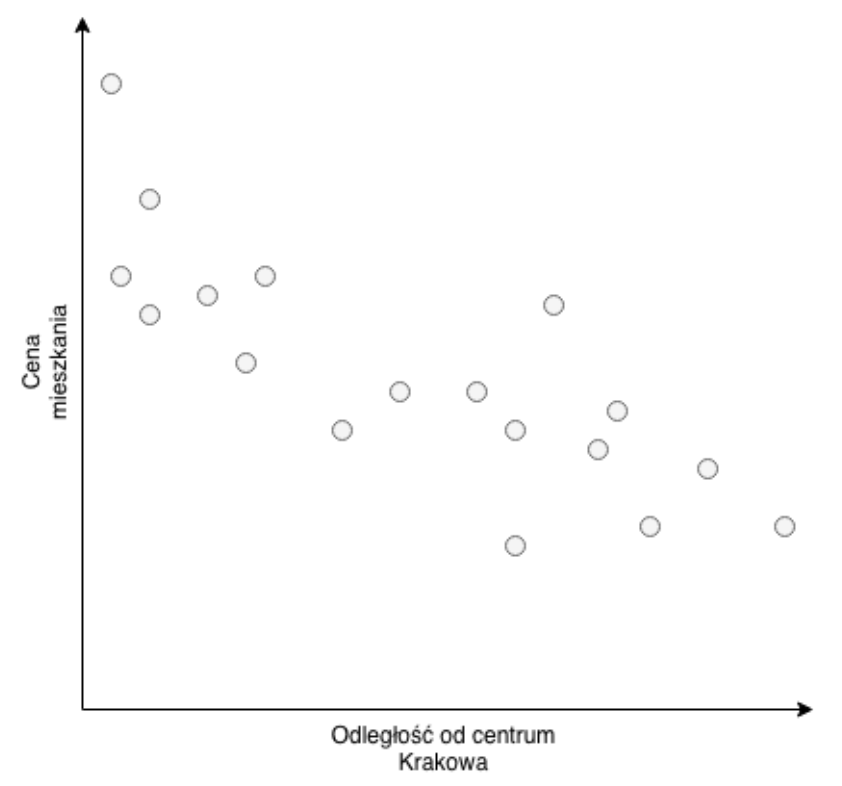
\includegraphics[width=8cm]{regression_dataset_example.png}
    \centering
    \caption{Wizualizacja przykładowego zbioru uczącego w problemie regresji}
    \end{figure}
    
    \item Klasyfikacja - należy również do uczenia nadzorowanego. Dane wyjściowe w problemach klasyfikacji mają postać dyskretną. Przykład: klasyfikacja nowotworu według wielkości guza.
    
    \begin{figure}[H]
    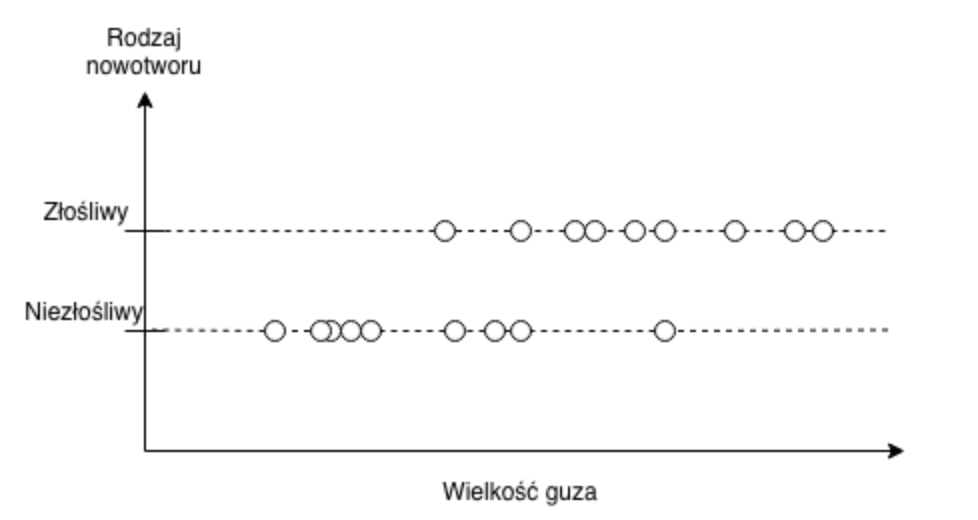
\includegraphics[width=8cm]{classification_dataset_example.png}
    \centering
    \caption{Wizualizacja przykładowego zbioru uczącego w problemie klasyfikacji}
    \end{figure}    
    
    \item Klasteryzacja - problem związany z uczeniem nienadzorowanym. Algorytm sam znajduje strukturę wprowadzonych danych i próbuje je rozdzielić na określoną (manualnie lub dynamicznie) liczbę klastrów.
    
    \begin{figure}[H]
    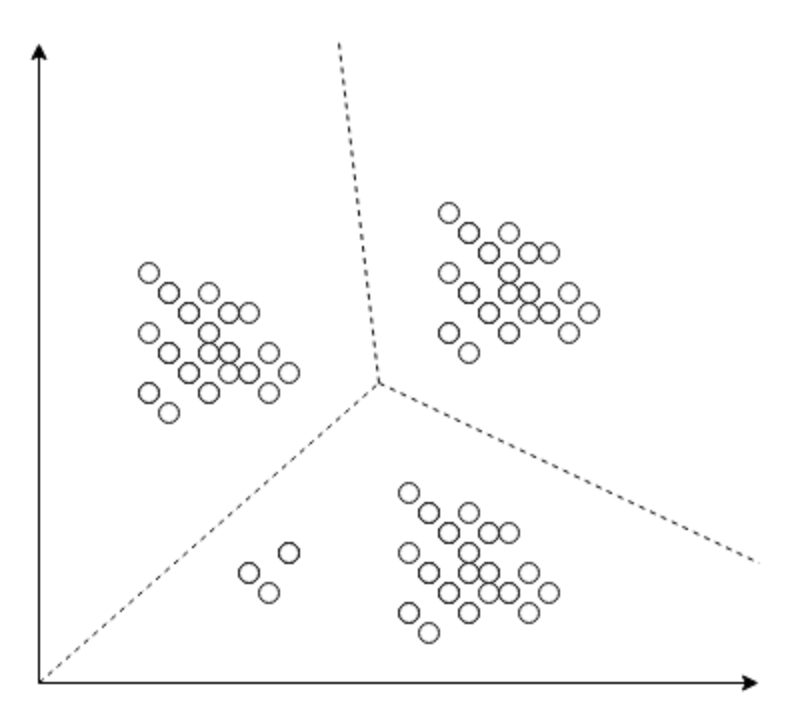
\includegraphics[width=8cm]{clustering_example.png}
    \centering
    \caption{Wizualizacja przykładowego procesu klasteryzacji}
    \end{figure}
    
\end{enumerate}

\subsection{Wybrane algorytmy uczenia maszynowego}

\subsubsection{Naiwny klasyfikator bayesowski}

Naiwny klasyfikator bayesowski jest oparty na metodach statystycznych, a dokładniej twierdzeniu Bayesa. Metoda ta zakłada, że wszystkie atrybuty (cechy) próbki mają być od siebie niezależne.

\textbf{Założenia}: Zbiór uczący składa się z n próbek, z których każda ma po m atrybutów. Każda próbka w zbiorze uczącym musi mieć również przypisaną klasę ze zbioru skończonego C. Posiadamy również jedną próbkę (określmy ją jako X) opisaną również przez m atrybutów (takich samych jak w zbiorze uczącym). Naszym zadaniem jest przypisanie odpowiedniej klasy ze zbioru C do próbki X.

\[ P(C_i|X) = \frac{P(X|C_i)P(C_i)}{P(X)} \]

\begin{center}
    $P(C_i|X)$ - prawdopodobieństwo, że X należy do klasy Ci
\end{center}

$P(X)$ jest dla wszystkich kategorii równe, dlatego możemy wykluczyć je z algorytmu.
Zakładamy również, że poszczególne kategorie mają równe prawdopodobieństwa 
$(C1 = C2 = ... = Cz)$, dzięki czemu nasze zadanie sprowadza się do maksymalizacji $P(X|C_i)$.

Wcześniej poczynione założenie mówiące, że wszystkie atrybuty są od siebie niezależne pozwala nam na kolejne przekształcenie równania do postaci:

\[ P(C_i|X) = \prod^{m}_{k=1} P(X_k|C_i) \]

Na tej podstawie jesteśmy już w stanie policzyć $P(Xk|C_i)$:

\begin{enumerate}
    \item Jeśli atrybut $X_k$ ma wartość ze zbioru skończonego (np. jest kategorią), wtedy liczymy prawdopodobieństwo, że próbki testowe należące do Ci mają atrybut k taki sam jak próbka X
    
    \item Jeśli atrybut jest wartością ciągłą, wtedy powinniśmy obliczyć $P(X_i|C)$ korzystając z funkcji rozkładu Gaussa.
\end{enumerate}

Wartość $P(C_i|X)$ musimy policzyć dla każdej klasy. Klasa dla której prawdopodobieństwo będzie największe, stanie się potencjalną kategorią próbki X.

Dużymi zaletami klasyfikatora Bayesa jest niska złożoność obliczeniowa i prostota. Natomiast należy cały czas pamiętać, że ten klasyfikator nie będzie dawał dobrych rezultatów, jeśli będą występowały znaczące zależności między atrybutami.

\subsection{Metoda k-średnich}

W problemach klasteryzacji jednym z najpopularniejszych obecnie algorytmów jest metoda k-średnich. Jego głównymi atutami są prostota oraz efektywność. Algorytm składa się z trzech ogólnych kroków:

\begin{enumerate}
    \item Inicjalizacja k centroidów (gdzie k jest dowolną liczbą całkowitą większą od zera).
    
    \item Przypisanie każdej próbki do jej najbliższego centroidu.

    \item Zmień pozycję centroidów biorąc po uwagę przypisania z punktu 2 (ustalona zostaje jako średnia wszystkich punktów przypisanych do centroidu). Jeśli pozycja się nie zmienia, zakończ działanie.
\end{enumerate}

Złożoność obliczeniową algorytmu k-means przyjmuje się jako: 

\[ O(t * k * n * d) \]

\begin{center}
t - ilość iteracji

k - ilość klastrów

n - ilość próbek

d - liczba wymiarów (dla pojedynczej próbki)
\end{center}

Pomimo liniowej złożoności algorytm k-średnich ma problemy z dużymi ilościami danych pochodzących z internetu, gdzie ilości próbek, klastrów oraz wymiarów są ogromne. Kolejnym problemem jest inicjalizacja klastrów. Wynik końcowy może się różnić w zależności od pierwotnych położeń centroidów.

\begin{figure}[H]
    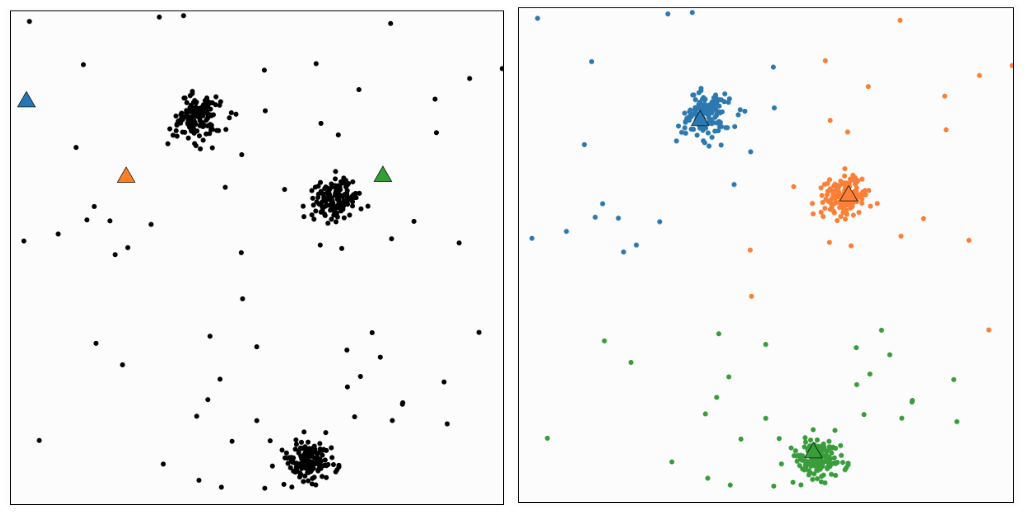
\includegraphics[width=10cm]{kmeans_example.png}
    \centering
    \caption{Przykład klasteryzacji (przed i po 8 iteracjach) na podstawie https://github.com/karanveerm/kmeans}
\end{figure} 
